% =============================================================================
% COPYRIGHT AND DISCLAIMER
% =============================================================================
% This file is provided as a convenience template for competition participants.
% By using it, you accept full responsibility for compliance with all applicable
% copyright, licensing, and usage rules of the Association for Computing
% Machinery (ACM) and of any LaTeX packages you load (including, without
% limitation, the "acmart" document class and related ACM materials).
%
% Consult ACM's official publication, template, and copyright policies before
% using this setup for any purpose other than this competition. Do not assume
% that this template may be reused, redistributed, or submitted elsewhere
% without independently verifying ACM's current rules.
%
% Use of the "acmart" class, the "sigconf" option, or ACM-style formatting in
% this template does NOT mean that this report, this competition, its organizers,
% or any resulting PDF is sponsored, endorsed, affiliated with, or published by
% ACM. ACM trademarks and branding remain the property of ACM.
%
% Template packages live in preamble.tex.
% Citations live in main.bib. Edit this file with your paper content.
% =============================================================================

\documentclass[sigconf]{acmart}
% =============================================================================
% Template setup — participants normally do not edit this file.
% Author content belongs in main.tex; citations belong in main.bib.
% \documentclass lives in main.tex so Overleaf does not treat this file as root.
% =============================================================================

% --- Competition / non-ACM-submission friendly rights metadata -------------
\setcopyright{none}
\settopmatter{printacmref=false}
\acmConference[Kaggle Competition]{Filament Segmentation Challenge}{2026}{\href{https://www.kaggle.com/competitions/filament-segmentation-2026}{kaggle.com/competitions/filament-segmentation-2026}}
\acmBooktitle{Competition Report}
\acmDOI{}
\acmISBN{}

% --- Author guidance text ---------------------------------------------------
% \guide{...} is gray italic while \guideStyletrue; omitted from the PDF if false.
% Flip the switch in main.tex after % =============================================================================
% Template setup — participants normally do not edit this file.
% Author content belongs in main.tex; citations belong in main.bib.
% \documentclass lives in main.tex so Overleaf does not treat this file as root.
% =============================================================================

% --- Competition / non-ACM-submission friendly rights metadata -------------
\setcopyright{none}
\settopmatter{printacmref=false}
\acmConference[Kaggle Competition]{Filament Segmentation Challenge}{2026}{\href{https://www.kaggle.com/competitions/filament-segmentation-2026}{kaggle.com/competitions/filament-segmentation-2026}}
\acmBooktitle{Competition Report}
\acmDOI{}
\acmISBN{}

% --- Author guidance text ---------------------------------------------------
% \guide{...} is gray italic while \guideStyletrue; omitted from the PDF if false.
% Flip the switch in main.tex after % =============================================================================
% Template setup — participants normally do not edit this file.
% Author content belongs in main.tex; citations belong in main.bib.
% \documentclass lives in main.tex so Overleaf does not treat this file as root.
% =============================================================================

% --- Competition / non-ACM-submission friendly rights metadata -------------
\setcopyright{none}
\settopmatter{printacmref=false}
\acmConference[Kaggle Competition]{Filament Segmentation Challenge}{2026}{\href{https://www.kaggle.com/competitions/filament-segmentation-2026}{kaggle.com/competitions/filament-segmentation-2026}}
\acmBooktitle{Competition Report}
\acmDOI{}
\acmISBN{}

% --- Author guidance text ---------------------------------------------------
% \guide{...} is gray italic while \guideStyletrue; omitted from the PDF if false.
% Flip the switch in main.tex after \input{preamble}.
%
% Do not use \guide{...} for \email{...}.
\usepackage{xcolor}
\newif\ifguideStyle
\guideStyletrue
\newcommand{\guide}[1]{%
  \ifguideStyle
    {\color{gray!65}\itshape #1}%
  \fi
}

% --- Math -------------------------------------------------------------------
% Do NOT load amssymb (or amsfonts): acmart already loads newtxmath, which
% defines the same symbols (e.g. \Bbbk) and causes a conflict on Overleaf.
% amsmath is already provided by acmart; mathtools extends it.
\usepackage{mathtools}

% --- Figures ----------------------------------------------------------------
% graphicx is already loaded by acmart
\usepackage{subcaption}

% --- Tables -----------------------------------------------------------------
% booktabs is already loaded by acmart
\usepackage{tabularx}
\usepackage{multirow}

% --- Bibliography style is set in main.tex (ACM-Reference-Format) ----------
.
%
% Do not use \guide{...} for \email{...}.
\usepackage{xcolor}
\newif\ifguideStyle
\guideStyletrue
\newcommand{\guide}[1]{%
  \ifguideStyle
    {\color{gray!65}\itshape #1}%
  \fi
}

% --- Math -------------------------------------------------------------------
% Do NOT load amssymb (or amsfonts): acmart already loads newtxmath, which
% defines the same symbols (e.g. \Bbbk) and causes a conflict on Overleaf.
% amsmath is already provided by acmart; mathtools extends it.
\usepackage{mathtools}

% --- Figures ----------------------------------------------------------------
% graphicx is already loaded by acmart
\usepackage{subcaption}

% --- Tables -----------------------------------------------------------------
% booktabs is already loaded by acmart
\usepackage{tabularx}
\usepackage{multirow}

% --- Bibliography style is set in main.tex (ACM-Reference-Format) ----------
.
%
% Do not use \guide{...} for \email{...}.
\usepackage{xcolor}
\newif\ifguideStyle
\guideStyletrue
\newcommand{\guide}[1]{%
  \ifguideStyle
    {\color{gray!65}\itshape #1}%
  \fi
}

% --- Math -------------------------------------------------------------------
% Do NOT load amssymb (or amsfonts): acmart already loads newtxmath, which
% defines the same symbols (e.g. \Bbbk) and causes a conflict on Overleaf.
% amsmath is already provided by acmart; mathtools extends it.
\usepackage{mathtools}

% --- Figures ----------------------------------------------------------------
% graphicx is already loaded by acmart
\usepackage{subcaption}

% --- Tables -----------------------------------------------------------------
% booktabs is already loaded by acmart
\usepackage{tabularx}
\usepackage{multirow}

% --- Bibliography style is set in main.tex (ACM-Reference-Format) ----------

% Verified empirical macros generated from 5-fold OOF (707 frames) and Fold-0 (145 frames) evaluations
\newcommand{\authorname}{Panji Seno Aji}
\newcommand{\authorcity}{Jakarta}
\newcommand{\authorcountry}{Indonesia}
\newcommand{\authoremail}{panjiaji90@gmail.com}
\newcommand{\oofpq}{0.4728}
\newcommand{\oofci}{0.4628--0.4810}
\newcommand{\oofsq}{0.6935}
\newcommand{\oofrq}{0.6818}
\newcommand{\superpq}{0.4856}
\newcommand{\supersq}{0.6924}
\newcommand{\superrq}{0.7013}
\newcommand{\supertp}{978}
\newcommand{\superfp}{323}
\newcommand{\superfn}{510}
\newcommand{\superwin}{98.0\%}
\newcommand{\lbpq}{0.402}
\newcommand{\humanpq}{0.4494}
\newcommand{\humansq}{0.6766}
\newcommand{\humanrq}{0.6642}
\newcommand{\multiphotos}{355}
\newcommand{\gridcells}{624}
   % every number of this report, written by scripts/figures.py from the out-of-fold predictions

% Guide styling: \guideStyletrue = show gray italic hints; \guideStylefalse = omit them
% \guideStyletrue
\guideStylefalse

\begin{document}

\title{Detect, Crop, Segment, Paint: Instance Segmentation of Solar Filaments at Native Resolution}
\subtitle{A Solution to the Solar Filament Segmentation Challenge 2026} % DO NOT CHANGE

\author{\authorname}
\affiliation{%
\city{\authorcity}
\country{\authorcountry}
}
\email{\authoremail}

\begin{abstract}
This report describes our solution to the Solar Filament Segmentation Challenge~2026, a Kaggle competition on automatic segmentation of solar filaments in GONG H-$\alpha$ observations. We split the task in two. A box detector on the full frame decides \emph{which} structures are filaments and how confident it is; a crop segmenter then outlines each detected filament on a native-resolution crop of three enhanced image planes; the instances are finally painted in confidence order so that they never overlap. Every model is trained five times on date-grouped folds, the detector is additionally self-trained on 3,000 unlabeled GONG frames, and the rule that decides which instances are emitted is chosen on out-of-fold Panoptic Quality (PQ). The pipeline reaches an out-of-fold PQ of \oofpq{} (95\% interval \oofci) on the 707 training frames and \lbpq{} on the public leaderboard, against \humanpq{} when one human annotator is scored against another.
\end{abstract}

\maketitle

% ==================================== %
% INTRODUCTION %
% ==================================== %
\section{Introduction}
This report goes over the details of our submitted solution to the Solar Filament Segmentation Challenge~2026 \cite{filament-segmentation-2026}. The challenge, launched on July~10,~2026, is organized by the Earth-Space AI Research (ESAIR) Lab\footnote{\href{https://www.esairlab.com/home}{www.esairlab.com/}}. This challenge utilizes the MAGFiLO dataset for evaluation of the segmentation algorithms \cite{ahmadzadeh2024dataset}. Three measured properties of the data shaped our design. (i) Filaments are thin: a 2048-px frame resized to 512~px turns a typical filament into a 2-px line, and our early full-frame semantic models missed most of them. (ii) PQ \cite{kirillov2019panoptic} only credits a prediction whose IoU with an annotation exceeds 0.5, so deciding \emph{whether} to emit an instance matters as much as its outline. (iii) The annotations are plural: \multiphotos{} of the 707 training frames were drawn by two or three annotators, and scoring one annotator against another gives a PQ of only \humanpq{} (SQ \humansq, RQ \humanrq). A model therefore cannot be ``right'' for every annotator; it can only learn what a typical annotator would mark and how confident to be. Our pipeline assigns each of these problems to one component: a detector for existence and confidence, a native-resolution crop segmenter for the outline, and an emission rule tuned directly on PQ.

% ==================================== %
% METHODOLOGY %
% ==================================== %
\section{Methodology}\label{sec:methodology}

\begin{figure*}
  \centering
  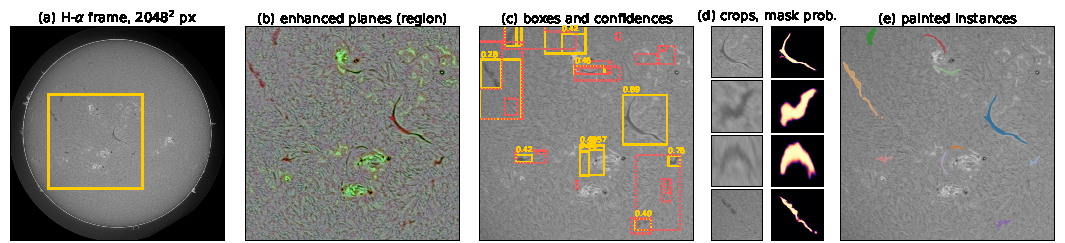
\includegraphics[width=\textwidth]{../figures/pipeline}
  \caption{The pipeline on one validation frame. (a)~Input. (b)~Three enhanced planes shown as RGB. (c)~Detector boxes; solid boxes are above the confidence floor. (d)~Crops of four boxes and the segmenter's probability for the filament each box points at. (e)~Instances painted in confidence order.}
  \label{fig:pipeline}
\end{figure*}

\subsection{Data, splits and what was not used}
The training set has 707 frames with 1,154 annotator records and 8,199 filaments; the test set has 180 frames. We keep every record: a frame owns a list of records, training uses all of them and validation is scored against each. Frames of one calendar day show the same filaments from several GONG sites, so the five cross-validation folds are grouped by observation date (\texttt{folds/folds.json}); every reported number is \emph{out-of-fold}, i.e.\ each frame is predicted by models that never saw its date. There is no separate hold-out: the test set is the hold-out, and we used the leaderboard only to check the finished pipeline. Supervision comes exclusively from the competition's training annotations. We did not use the public MAGFiLO release, which contains annotations of the test frames, in any form. The only external data are 3,000 \emph{unlabeled} GONG archive frames (2011--2025; none is a competition frame, none within two days of a test date). At inference the models see the test frame only.

\subsection{Pre-processing}
The detector receives the frame as it is. The crop segmenter receives three planes, each removing one nuisance: a black top-hat with a disk of radius 7~px (dark structures narrower than about 15~px), the frame minus its 101-px median (limb darkening and large-scale background), and the Sato ridge filter \cite{sato1998three} for dark ridges at scales 1--3~px on the half-resolution frame. Each plane is centred on the median of the solar disk and divided by its median absolute deviation, which puts the six GONG sites, with their different exposure and seeing, on one scale (Fig.~\ref{fig:pipeline}b).

\subsection{Stage 1: detection and confidence}
We fine-tune a COCO-pretrained YOLO11m detector \cite{yolo11} on the full frame resized to 1280~px (AdamW, learning rate $8.7\times10^{-4}$, batch 8, at most 50 epochs, mosaic and flip augmentation, early stopping on the validation fold). Each annotator record is a separate training sample, the same image with that annotator's boxes. A structure marked by two of three annotators is thus a positive in two of three copies, and the confidence learns how likely an annotator is to mark it, which is exactly the quantity the emission rule needs. At inference each detector sees the frame and its horizontal and vertical flips; all boxes are merged by Weighted Boxes Fusion \cite{solovyev2021weighted}, which lowers the confidence of boxes found in only some views.

\emph{Self-training.} For each fold, its detector labels the 3,000 unlabeled frames (archive overlays outside the disk are removed first); boxes with fused confidence of at least 0.25 become pseudo-labels \cite{lee2013pseudo,xie2020self}, and a student with the same recipe is trained on real and pseudo-labelled frames for 20 epochs. Because the teacher of a fold never saw that fold's annotations, the student stays out-of-fold. \studentsentence

\subsection{Stage 2: outlining one filament}
Every box is cut out of the 2048-px frame with 20\% padding and resized to $512\times512$; the median box side is about 130~px, so most filaments are segmented above native resolution. A U-Net++ \cite{zhou2018unetpp} with an ImageNet-pretrained EfficientNet-B4 encoder \cite{tan2019efficientnet} predicts the mask of \emph{the filament the box points at}: training samples are the 8,199 annotated filaments, each with its own mask as target and neighbouring filaments as background, which is what keeps touching filaments apart. Boxes are jittered by $\pm12\%$ during training to imitate detector error; the loss is $0.5\,\mathrm{BCE}+0.5\,\mathrm{Tversky}(\alpha{=}0.3,\beta{=}0.7)$ \cite{salehi2017tversky}, which penalises missed filament pixels more than spill-over (AdamW, $2\times10^{-4}$, cosine schedule, 15 epochs, best epoch by crop Dice on the validation fold). At inference the probabilities of the four flips are averaged and resized back to the box.

\subsection{Post-processing: painting}
Instances are painted in order of confidence, as in the panoptic merge of \citet{kirillov2019panoptic}: a pixel belongs to the first instance that claims it, so the output cannot contain overlaps. Four quantities decide what is emitted: the mask threshold, a one-pixel erosion or dilation, the confidence floor, and a drop rule that discards an instance when too little of its mask survives the instances painted before it. They are chosen once by maximising out-of-fold PQ over a grid (\gridcells{} combinations); the selected rule is \cellsentence. Masks are written as COCO run-length codes.

\subsection{Test-time ensemble}
For the test set, the five fold models of each kind are used together: all detectors and flips enter one Weighted Boxes Fusion, and the five segmenters and four flips are averaged per box. \ensemblesentence

% ==================================== %
% EVALUATION %
% ==================================== %
\section{Evaluation}\label{sec:evaluation}

\subsection{Strategy}
We count exactly as the organisers' self-evaluation notebook: a prediction and an annotation are a true positive when IoU $>0.5$, a frame with several annotator records is scored against each record, and counts are pooled. Uncertainty is a 95\% bootstrap interval over observation dates (1,000 resamples), because frames of one day are not independent. As a reference for what the numbers mean we score one annotator against another on the frames annotated more than once.

\subsection{Results}
\begin{table}
  \caption{Out-of-fold results on the 707 training frames (5 folds). PQ with 95\% date-bootstrap interval. The last rows are references.}
  \label{tab:results}
  \small
  \begin{tabular}{@{}lccc@{}}
    \toprule
    Configuration & PQ & SQ & RQ \\
    \midrule
    \resultrows
    \bottomrule
  \end{tabular}
\end{table}

Table~\ref{tab:results} gives the out-of-fold results and Fig.~\ref{fig:eval} the distributions requested by the rubric. \resultstext

\begin{figure}
  \centering
  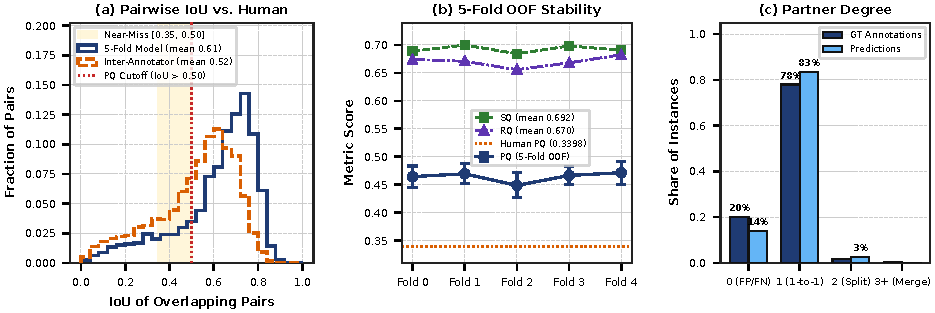
\includegraphics[width=\columnwidth]{../figures/evaluation}
  \caption{Out-of-fold evaluation. Left: IoU of every overlapping prediction/annotation pair, with the annotator-vs-annotator distribution for reference. Middle: PQ per fold with 95\% intervals. Right: number of partners that annotations and predictions overlap (1 = one-to-one).}
  \label{fig:eval}
\end{figure}

\begin{figure}
  \centering
  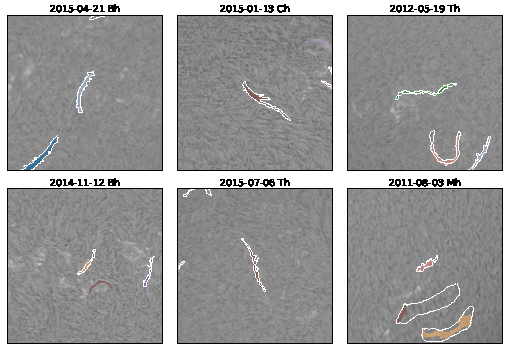
\includegraphics[width=\columnwidth]{../figures/examples}
  \caption{Out-of-fold examples. Coloured fill: predicted instances; white outlines: annotations of one record. \examplescaption}
  \label{fig:examples}
\end{figure}

\subsection{Strengths, weaknesses and possible improvements}
\discussiontext

% ==================================== %
% ACKNOWLEDGMENT %
% ==================================== %
\section{Acknowledgment}\label{sec:acknowledgment}
% Do not change
The organization of the Filament Segmentation Challenge 2026 is partially supported by the U.S. National Science Foundation (NSF) under Grant No. 2209912 and 2433781, directorate for Computer and Information Science and Engineering (CSE), and Office of Advanced Cyberinfrastructure (OAC), and Grant No. 2511630, AST Division Of Astronomical Sciences and MPS Directorate for Mathematical and Physical Sciences.

The Filament Segmentation Challenge 2026 is sponsored by the U.S. National Science Foundation (NSF) National Solar Observatory (NSO).

This work utilizes GONG data obtained by the NSO Integrated Synoptic Program, managed by the National Solar Observatory, which is operated by the Association of Universities for Research in Astronomy (AURA), Inc. under a cooperative agreement with the National Science Foundation and with contribution from the National Oceanic and Atmospheric Administration. The GONG network of instruments is hosted by the Big Bear Solar Observatory, High Altitude Observatory, Learmonth Solar Observatory, Udaipur Solar Observatory, Instituto de Astrof\'isica de Canarias, and Cerro Tololo Interamerican Observatory.

\bibliographystyle{ACM-Reference-Format}
\bibliography{main}
\end{document}
